%%%%%%%%%%%%%%%%%%%%%%%%%%%%%%%%%%%%%%%%%%%%%%%%%%
% Basic setup. Most papers should leave these options alone.
\documentclass[a4paper,fleqn,usenatbib]{mnras}

% MNRAS is set in Times font. If you don't have this installed (most LaTeX
% installations will be fine) or prefer the old Computer Modern fonts, comment
% out the following line
%\usepackage{newtxtext,newtxmath}
% Depending on your LaTeX fonts installation, you might get better results with one of these:
%\usepackage{mathptmx}
\usepackage{amsmath}	% Advanced maths commands
\usepackage{txfonts}

\setcounter{secnumdepth}{4}

% Use vector fonts, so it zooms properly in on-screen viewing software
% Don't change these lines unless you know what you are doing
\usepackage[T1]{fontenc}
\usepackage{ae,aecompl}


%%%%% AUTHORS - PLACE YOUR OWN PACKAGES HERE %%%%%

% Only include extra packages if you really need them. Common packages are:
\usepackage{graphicx}	% Including figure files
\usepackage{amssymb}	% Extra maths symbols

%%%%%%%%%%%%%%%%%%%%%%%%%%%%%%%%%%%%%%%%%%%%%%%%%%

%%%%% AUTHORS - PLACE YOUR OWN COMMANDS HERE %%%%%

% Please keep new commands to a minimum, and use \newcommand not \def to avoid
% overwriting existing commands. Example:
%\newcommand{\pcm}{\,cm$^{-2}$}	% per cm-squared
\newcommand{\jr}[1]{{\color{red} \bf JR: #1}}   %John Regan
\newcommand{\bwo}[1]{{\color{red} \bf BWO: #1}}   %Brian O'Shea
\newcommand{\addcite}[1]{{\color{blue} (\bf REF: #1)}}   %

%%%%%%%%%%%%%%%%%%%%%%%%%%%%%%%%%%%%%%%%%%%%%%%%%%

%%%%%%%%%%%%%%%%%%% TITLE PAGE %%%%%%%%%%%%%%%%%%%

% Title of the paper, and the short title which is used in the headers.
% Keep the title short and informative.
\title[Grackle]{Grackle: a Chemistry and Cooling
  Library for Astrophysics}

% The list of authors, and the short list which is used in the headers.
% If you need two or more lines of authors, add an extra line using \newauthor
\author[B.D. Smith et al.]
       {Britton D. Smith,$^{1}$\thanks{E-mail: brittonsmith@gmail.com
           (BDS)},
        Greg L. Bryan$^{2,3}$,
        Simon C. O. Glover$^{4}$,
        Nathan J. Goldbaum$^{5}$, \newauthor
        Matthew J. Turk$^{6,7}$,
        John Regan$^{8,9}$,
        John H. Wise$^{10}$,
        Hsi-Yu Schive$^{5}$,
        Tom Abel$^{11,12}$, \newauthor
        Andrew Emerick$^{2,13}$,
        Brian W. O'Shea$^{14,15,16}$,
        Peter Anninos$^{17}$, \newauthor
        Cameron B. Hummels$^{18}$,
        and Sadegh Khochfar$^{1}$\\
% List of institutions
$^{1}$Institute for Astronomy, University of Edinburgh, Royal
Observatory, Edinburgh EH9 3HJ, UK\\
$^{2}$Columbia University, Department of Astronomy, New York, NY,
10025, USA\\
$^{3}$Simons Center for Computational Astrophysics, New York, NY,
USA\\
$^{4}$Universit\"{a}t Heidelberg, Zentrum f\"{u}r Astronomie, Institut
f\"{u}r Theoretische Astrophysik, Albert-Ueberle-Stra{\ss}e 2, \\69120
Heidelberg, Germany\\
$^{5}$National Center for Supercomputing Applications, University of
Illinois, Urbana-Champaign, IL, 61820, USA\\
$^{6}$School of Information Sciences, University of Illinois,
Urbana-Champaign, IL, 61820, USA\\
$^{7}$Department of Astronomy, University of Illinois,
Urbana-Champaign, IL, 61820, USA\\
$^{8}$Institute for Computational Cosmology, Durham University, South
Road, Durham, DH1 3LE, UK \\
$^{9}$School of Mathematical Sciences, Dublin City University, Dublin,
Ireland \\
$^{10}$Center for Relativistic Astrophysics, Georgia Institute of
Technology, 837 State Street, Atlanta, GA 30332, USA\\
$^{11}$Kavli Institute for Particle Astrophysics and Cosmology,
Stanford University, Menlo Park, CA 94025, USA\\
$^{12}$Department of Physics, Stanford University, Stanford, CA 94305,
USA\\
$^{13}$American Museum of Natural History, Department of Astrophysics,
New York, NY, USA\\
$^{14}$Department of Physics and Astronomy, Michigan State University,
East Lansing, MI 48824, USA\\
$^{15}$Department of Computational Mathematics, Science and
Engineering, Michigan State University, East Lansing, MI 48824, USA\\
$^{16}$JINA: Joint Institute for Nuclear Astrophysics, Michigan State
University, East Lansing, MI 48824, USA\\
$^{17}$Lawrence Livermore National Laboratory, Livermore, CA 94550\\
$^{18}$California Institute of Technology, Pasadena, CA 91125, USA\\
}

% These dates will be filled out by the publisher
\date{Accepted XXX. Received YYY; in original form ZZZ}

% Enter the current year, for the copyright statements etc.
\pubyear{2016}

% Don't change these lines
\begin{document}
\label{firstpage}
\pagerange{\pageref{firstpage}--\pageref{lastpage}}
\maketitle

% Abstract of the paper
\begin{abstract}
We present the \texttt{Grackle} chemistry and cooling library for
astrophysical simulations and models.  \texttt{Grackle} provides
a treatment of non-equilibrium primordial chemistry and cooling for H, D, and He
species, including H$_{2}$ formation on dust grains; tabulated
primordial and metal cooling; multiple UV background models; and
support for radiation transfer and arbitrary heat sources.  The
library has an easily implementable interface for simulation codes
written in C, C++, and Fortran as well as a Python interface with
added convenience functions for semi-analytical models.  As an
open-source project, \texttt{Grackle} provides a community resource
for accessing and disseminating astrochemical data and numerical
methods.  We present the full details of the core functionality, the
simulation and Python interfaces, testing infrastructure, performance,
and range of applicability.  {\bf \texttt{Grackle} is a fully open-source
project and new contributions are welcome.}
\end{abstract}

% Select between one and six entries from the list of approved keywords.
% Don't make up new ones.
\begin{keywords}
astrochemistry -- methods: numerical -- galaxies: formation
\end{keywords}

%%%%%%%%%%%%%%%%%%%%%%%%%%%%%%%%%%%%%%%%%%%%%%%%%%

%%%%%%%%%%%%%%%%% BODY OF PAPER %%%%%%%%%%%%%%%%%%

\section{Introduction} \label{sec:intro}

\subsection{Why is chemistry/radiative cooling necessary in
  simulations?}

\subsection{Why is a multi-code library a good thing?}


%\section{Chemistry and Cooling Methods} \label{sec:physics}


% ========== Primoridal Chemistry =========

\section{Primordial Chemistry} \label{sec:primordial_chemistry}
The treatment of primordial chemistry (i.e.\ the chemistry of metal-free gas) used in Grackle is closely based on the
treatment in the Enzo AMR code \citep{2014ApJS..211...19B}, although Grackle accounts for a few processes that are not included 
in the latest version of Enzo available at the time of writing (version 2.4). The Enzo primordial chemistry itself is based 
originally on the work of \citet{1997NewA....2..181A} and \citet{1997NewA....2..209A}, although the current version has been
modified substantially compared to the original Abel~et~al.\ network. In this section, we describe in detail the chemistry 
included in Grackle and discuss how the resulting set of chemical rate equations is solved. 

\subsection{Chemistry Network} \label{sec:network}
Grackle provides three different primordial chemistry networks, differing in the number of chemical species that they include. 
The choice of chemical network is controlled by the \texttt{primordial\_chemistry} parameter. Setting \texttt{primordial\_chemistry = 1} selects the
six species network, which tracks the abundances of the species H, H$^{+}$, He, He$^{+}$, He$^{++}$ and e$^{-}$ and is 
designed for modelling atomic and/or ionized gas. Setting \texttt{primordial\_chemistry = 2} selects the nine species network. This
includes all of the species and reactions included in the six species network, but adds molecular hydrogen (H$_2$), plus the
two ions primarily responsible for its formation in primordial gas (H$^{-}$ and H$_{2}^{+}$). Finally, setting \texttt{primordial\_chemistry = 3}
selects the twelve species network, which is an extension of the nine species model that includes D, D$^{+}$ and HD.

\begin{table}
\caption{Chemical reactions in the six species network \label{tab:six}}
\begin{tabular}{lclcc}
\hline
\multicolumn{3}{c}{Reaction} & \multicolumn{2}{c}{Reference} \\
& & & Data & Fit \\
\hline
${\rm H + e^{-}}$ & $\rightarrow$ & $\rm{H^{+} + e^{-} + e^{-}}$ & 1 & 2 \\
${\rm H^{+} + e^{-}}$ & $\rightarrow$ & $\rm{H + \gamma} $ & 3 & 2, 4\\
${\rm He + e^{-}}$ & $\rightarrow$ & ${\rm He^{+} + e^{-} + e^{-}}$ & 1 & 2 \\
${\rm He^{+} + e^{-}}$ & $\rightarrow$ & ${\rm He + \gamma}$ & 5, 6 & 4, 6, 7 \\
${\rm He^{+} + e^{-}}$ & $\rightarrow$ & ${\rm He^{++} + e^{-} + e^{-}}$ & 1 & 2 \\
${\rm He^{++} + e^{-}}$ & $\rightarrow$ & ${\rm He^{+} + \gamma}$ & 3, 8 & 4, 9 \\
${\rm H + H}$ & $\rightarrow$ & ${\rm H^{+} + e^{-} + H}$ & 10 & 11 \\
${\rm H + He}$ & $\rightarrow$ & ${\rm H^{+} + e^{-} + He}$ & 12 & 11 \\
${\rm H + \gamma}$ & $\rightarrow$ & ${\rm H^{+} + e^{-}}$ & 13 & --- \\
${\rm He + \gamma}$ & $\rightarrow$ & ${\rm He^{+} + e^{-}}$ & 13 & --- \\
${\rm He^{+} + \gamma}$ & $\rightarrow$ & ${\rm He^{++} + e^{-}}$ & 13 & --- \\
\hline
\end{tabular}
\\ Key: 1 -- \citet{1987ephh.book.....J}; 2 -- \citet{1997NewA....2..181A}; 3 -- \citet{1992ApJ...387...95F}; 4 -- \citet{1997MNRAS.292...27H}; 5 -- \citet{1960MNRAS.121..471B}; 6 -- \citet{1973A&A....25..137A}; 7 -- \citet{1981MNRAS.197..553B}; 8 -- \citet{1978ppim.book.....S}; 9 -- \citet{1992ApJS...78..341C}; 10 -- \citet{1987PhRvA..36.3100G}; 11 -- \citet{1991ApJS...76..759L}; 12 -- \citet{1981JChPh..74..314V}; 13 -- see Section~\ref{section:radback}
\end{table}

The reactions included in the six species network are listed in Table~\ref{tab:six}. The rate coefficients for these reactions are implemented in
Grackle using simple temperature-dependent analytical fits. In the Table, we list the references from which we take these fits, and also the 
references that are the original sources of the theoretical or experimental  data on which these fits are based.

A few of the reactions listed in Table~\ref{tab:six} deserve further comment:
\begin{enumerate}
\item[(i)] By default, the recombination of
H$^{+}$, He$^{+}$ and He$^{++}$ is modelled using the case A recombination rate coefficients. However, the case B
rate coefficients can instead be selected by setting casebrates = 1. The additional complication that photons from the recombination of
He$^{+}$ can bring about the photoionization of hydrogen \citep[discussed in some detail in][]{1989agna.book.....O} is not accounted
for, but in most circumstances this will only lead to a small error in the H$^{+}$ and He$^{+}$ abundances. 
\item[(ii)] The rates of the photoionization reactions are not calculated internally by Grackle, but instead are specified in an input data file,
as described in more detail in Section~\ref{section:radback}.
\item[(iii)] The six species network implemented in Grackle includes two additional reactions that were not part of the original \citet{1997NewA....2..181A}
six species network: the collisional ionization of H by collisions with H and He atoms. Often, these reactions are unimportant. However, they 
can become competitive with the collisional ionization of H by electrons if the fractional ionization of the gas is very low \citep[see e.g.][for an example of when this can be important]{2015MNRAS.451.2082G}.
\end{enumerate}

\begin{table}
\caption{Chemical reactions in the nine species network \label{tab:nine}}
\begin{tabular}{lclcc}
\hline
\multicolumn{3}{c}{Reaction} & \multicolumn{2}{c}{Reference} \\
& & & Data & Fit \\
\hline
${\rm H + e^{-}}$ & $\rightarrow$ & ${\rm H^{-} + \gamma}$ & 1 & 2 \\
${\rm H^{-} + H}$ & $\rightarrow$ & ${\rm H_{2} + e^{-}}$ & 3 & 3 \\
${\rm H + H^{+}}$ & $\rightarrow$ & ${\rm H_{2}^{+} + \gamma}$ & 4 & 5 \\
${\rm H_{2}^{+} + H}$ & $\rightarrow$ & ${\rm H_{2} + H^{+}}$ & 6 & 6 \\
${\rm H_{2} + H^{+}}$ & $\rightarrow$ & ${\rm H_{2}^{+} + H}$ & 7 & 8 \\
${\rm H_{2} + e^{-}}$ & $\rightarrow$ & ${\rm H + H + e^{-}}$ & 9 & 9 \\
${\rm H_{2} + H}$ & $\rightarrow$ & ${\rm H + H + H}$ & 10 & 10 \\
${\rm H^{-} + e^{-}}$ & $\rightarrow$ & ${\rm H + e^{-} + e^{-}}$ & 11 & 12 \\
${\rm H^{-} + H}$ & $\rightarrow$ & ${\rm H + e^{-} + H}$ & 11 & 12 \\
${\rm H^{-} + H^{+}}$ & $\rightarrow$ & ${\rm H + H}$ & 13 & 14 \\
${\rm H^{-} + H^{+}}$ & $\rightarrow$ & ${\rm H_{2}^{+} + e^{-}}$ & 15 & 12, 16 \\
${\rm H_{2}^{+} + e^{-}}$ & $\rightarrow$ & ${\rm H + H}$ & 17 & 12 \\
${\rm H_{2}^{+} + H^{-}}$ & $\rightarrow$ & ${\rm H_{2} + H}$ & 18 & 18 \\ 
${\rm H + H + H}$ & $\rightarrow$ & ${\rm H_{2} + H}$ & 19  & 19  \\
${\rm H + H + H_{2}}$ & $\rightarrow$ & ${\rm H_{2} + H_{2}}$ & 20, 21 & 22 \\
${\rm H^{-} + \gamma}$ & $\rightarrow$ & ${\rm H + e^{-}}$ & 23 & --- \\
${\rm H_{2}^{+} + \gamma}$ & $\rightarrow$ & ${\rm H + H^{+}}$ & 23 & --- \\
${\rm H_{2} + \gamma}$ & $\rightarrow$ & ${\rm H_{2}^{+} + e^{-}}$ & 23 & --- \\
${\rm H_{2}^{+} + \gamma}$ & $\rightarrow$ & ${\rm H^{+} + H^{+} + e^{-}}$ & 23 & --- \\
${\rm H_{2} + \gamma}$ & $\rightarrow$ & ${\rm H + H}$ & 23 & --- \\
${\rm H + H + grain}$ & $\rightarrow$ & ${\rm H_{2} + grain}$ & --- & 24$^{*}$ \\
\hline
\end{tabular}
\\ Note: the nine species network also includes all of the reactions listed in Table~\ref{tab:six}.
\\ Key: 1 -- \citet{1979MNRAS.187P..59W}; 2 --
\citet{1998ApJ...509....1S}; 3 -- \citet{2010Sci...329...69K}; 4 --
\citet{1976PhRvA..13...58R}; 5 -- \citet{2015MNRAS.446.3163L}; 6 --
\citet{1979JChPh..70.2877K}; 7 -- \citet{2002PhRvA..66d2717K}; 8 ---
\citet{2004ApJ...606L.167S,2004ApJ...607L.147S}; 9 --
\citet{2002PPCF...44.1263T}; 10 -- \citet{1996ApJ...461..265M}; 11 --
\citet{1987ephh.book.....J}; 12 -- \citet{1997NewA....2..181A}; 13 --
\citet{1986JPhB...19L..31F}; 14 -- \citet{1999MNRAS.304..327C}; 15 --
\citet{1978JPhB...11L.671P}; 16 -- \citet{1987ApJ...318...32S}; 17 --
\citet{1994ApJ...424..983S}; 18 -- \citet{1987IAUS..120..109D}; 19 --
See text; 20 -- \citet{1962JChPh..36.2923S}; 21 --
\citet{1970JChPh..53.4395H}; 22 -- \citet{1983JPCRD..12..531C}; 23 --
see Section~\ref{section:radback}; 24 -- \citet{1985ApJ...291..722T,
  2000ApJ...534..809O}; * - This reaction included as an additional
option when metals are present.
\end{table}

The nine species network includes all of the reactions in Table~\ref{tab:six} plus the additional reactions listed in Table~\ref{tab:nine}. Again,
a couple of reactions deserve further discussion:
\begin{enumerate}
\item[(i)] The treatment of H$_{2}$ collisional dissociation by H atom collisions now used in Grackle is taken from \citet{1996ApJ...461..265M} and 
accounts for both the temperature and the density dependence of this process. It therefore remains valid in the high density limit, where the H$_{2}$
level populations approach their local thermodynamical equilibrium (LTE) values. This is important, because H$_{2}$ is far more susceptible to
collisional dissociation in this limit than when it is solely in the vibrational ground state. It should also be noted that the treatment of this process
in Grackle accounts for effects of dissociative tunneling as well as direct collisional dissociation; previously, Enzo only accounted for the latter
process and hence underestimated the dissociation rate at low temperatures \citep{2014MNRAS.443.1979L,2015MNRAS.451.2082G}
\item[(ii)] In view of the considerable uncertainty in the rate of the three-body reaction
\begin{equation}
{\rm H + H + H} \rightarrow {\rm H_{2} + H},
\end{equation}
discussed in detail in \citet{2008AIPC..990...25G} and \citet{2011ApJ...726...55T}, Grackle provides several different rate coefficients for this process. The user can
select which of these rate coefficients to adopt by means of the three\_body\_rate parameter. The options are
\begin{enumerate}
\item[{\bf 0}:]  Rate coefficient from \citet{2002Sci...295...93A}, based on an extrapolation from low temperature calculations by \citet{1987JChPh..87..314O}. This is the default option.
\item[{\bf 1}:]  Rate coefficient from \citet{1983ApJ...271..632P}, derived using detailed balance applied to the H$_{2}$ collisional dissociation rate measured by \citet{1967JChPh..47...54J}.
\item[{\bf 2}:]  Rate coefficient recommended by \citet{1983JPCRD..12..531C}, based on a survey of the experimental data available at that time. 
\item[{\bf 3}:]  Rate coefficient from \citet{2007MNRAS.377..705F}, also derived from \citet{1967JChPh..47...54J} using detailed balance, but with a different treatment of the H$_{2}$ partition
function. 
\item[{\bf 4}:]  Rate coefficient from \citet{2008AIPC..990...25G}, derived from the \citet{1996ApJ...461..265M} high-density H$_2$ collisional dissociation rate using detailed balance
\item[{\bf 5}:]  Rate coefficient computed directly by \citet{2013ApJ...773L..25F}.
\end{enumerate}
\end{enumerate}

Finally, the twelve species network includes the reactions in Tables~\ref{tab:six} and \ref{tab:nine}, plus a small number of additional reactions involving
D$^{+}$, D and HD, listed in Table~\ref{tab:12}. The intent of the twelve species network is to allow the HD abundance of the gas to be tracked accurately,
since in cold gas HD can become a more effective coolant than H$_{2}$ despite its much lower fractional abundance \citep[see e.g.][]{2006MNRAS.366..247J,2008ApJ...685....8M}. It is therefore necessary to include only a small number of reactions, as the direct conversion of H$_{2}$ to HD by collisions with D$^{+}$ and D, together with the
corresponding inverse reactions generally dominate the production and destruction of HD.

Two reactions in the twelve species network require further discussion:
\begin{enumerate}
\item[(i)] The rate coefficient that we adopt for the reaction
\begin{equation}
{\rm HD + H} \rightarrow {\rm H_{2} + D}
\end{equation}
is an analytical fit presented in \citet{2002P&SS...50.1197G}, based on data from \citet{1959JChPh..31.1359S}. However, this fit blows up
at temperatures $T < 100$~K, yielding an unphysically large value for the rate coefficient. We therefore follow \citet{2007MNRAS.376..709R}
and \citet{2008ApJ...685....8M} and assume that the rate at $T < 100$~K is the same as the rate at $T = 100$~K. Note that as this reaction
proceeds extremely slowly at temperatures below as few hundred K, this is unlikely to be a significant source of error. 
\item[(ii)] We assume that the rate coefficient for the associative detachment of H$^{-}$ by D
\begin{equation}
{\rm D + H^{-} \rightarrow  HD + e^{-}}
\end{equation}
is the same as for the corresponding reaction between H and H$^{-}$, since measurements by \citet{2012PhRvA..86c2714M} suggest that
there is not a significant isotope effect for this reaction. However, in the solver, we multiply the rate coefficient by a factor of two when
computing the HD formation rate to account approximately for the contribution from the reaction
\begin{equation}
{\rm H + D^{-} \rightarrow  HD + e^{-}}.
\end{equation}
Note that we do not explicitly include this reaction in our network because it would require us to track the abundance of the D$^{-}$ ion,
thereby adding significant additional complexity to the model for only a marginal increase in accuracy.
\end{enumerate}

\begin{table}
\caption{Additional reactions included in the twelve species network \label{tab:12}}
\begin{tabular}{lclcc}
\hline
\multicolumn{3}{c}{Reaction} & \multicolumn{2}{c}{Reference} \\
& & & Data & Fit \\
\hline
${\rm H^{+} + D}$ & $\rightarrow$ & ${\rm H + D^{+}}$ & 1, 2 & 3 \\
${\rm D^{+} + H}$ & $\rightarrow$ & ${\rm D + H^{+}}$ & 1, 2 & 3 \\
${\rm H_{2} + D^{+}}$ & $\rightarrow$ & ${\rm HD + H^{+}}$ & 4 & 5 \\
${\rm HD + H^{+}}$ & $\rightarrow$ & ${\rm H_{2} + D^{+}}$ & 4 & 5 \\
${\rm H_{2} + D}$ & $\rightarrow$ & ${\rm HD + H}$ & 6 & 7 \\
${\rm HD + H}$ & $\rightarrow$ & ${\rm H_{2} + D}$ & 8 & 5, 9 \\
${\rm D + H^{-}}$ & $\rightarrow$ & ${\rm HD + e^{-}}$ & 10, 11 & 10  \\
\hline
\end{tabular}
\\ Note: the twelve species network also includes all of the reactions listed in Tables~\ref{tab:six} \& \ref{tab:nine}.
\\ Key: 1 -- \citet{1999PhRvL..83.4041I}; 2 -- \citet{2000PhRvA..62d2706Z}; 3 -- \citet{2002ApJ...566..599S};
4 -- \citet{1982sasp.nasa..304G}; 5 -- \citet{2002P&SS...50.1197G}; 6 -- \citet{2003PhRvL..91f3201M}; 7 -- \citet{2011ApJ...727..110C}; 
8 -- \citet{1959JChPh..31.1359S}; 9 -- \citet{2007MNRAS.376..709R}; 10 -- \citet{2010Sci...329...69K}; 11 -- \citet{2012PhRvA..86c2714M}
\end{table}

% ----------------------------------

\subsection{Solving and Updating the Network}

Chemical networks such as the ones described above are often challenging to evolve due to the very different time scales that various rates may have -- creation and destruction time scales can differ by orders of magnitude among the different species.   Such ``stiff" sets of equations are often solved with implicit methods, which permit longer timesteps.  Several packages exist to do this, and can even switch between methods for solving stiff and non-stiff equations, such as LSODAR (Hindmarsh 1983); however, for multi-dimensional simulations it is useful to have an implementation which is optimized for the case at hand.

Our kinetic network for solving the rate of change of species density $n_i$ has the general form
\begin{equation}
\frac{\partial n_i}{\partial t} = \sum_j \sum_l k_{jl} n_j n_l + \sum_j I_j n_j
\label{eq:rate_general}
\end{equation}
where $k_{jl}$ is the rate for reactions involving species $j$ and $l$ while $I_j$ is the appropriate radiative rate.  Note that in rare cases there may an additional term for three-body reactions.   To solve this kinetic network, Grackle follows closely the procedure described in \citet{1997NewA....2..209A} and \citet{2014ApJS..211...19B} by grouping creation and destruction rates to rewrite Eq.~\ref{eq:rate_general} as,
\begin{equation}
\frac{\partial n_i}{\partial t} = C_i(T, n_j) - D_i(T, n_j) n_i
\label{eq:rateCD}
\end{equation}
where $C_i$ represents the total creation rate of species $i$ (given the temperature $T$ and other species densities) while $D_i n_i$ is the destruction rate of the same species (which must be proportional to $n_i$), including both radiative and collisional processes.  Ideally, we would solve these ordinary differential equations using a higher order method; however, here we adopt a very simple low order backwards difference formula (BDF) due to its stability.  \citet{1997NewA....2..209A} explored a variety of higher-order solution techniques but found that this simple BDF scheme was generally more stable and competitive for the level of accuracy required.  In particular, the BDF version of Equation~\ref{eq:rateCD} is:
\begin{equation}
n^{t + \Delta t} = \frac{C^{t+\Delta t} \Delta t + n^t}{1 + D^{t+\Delta t} \Delta t}
\label{eq:rate_BDF}
\end{equation}
Unfortunately, we are not able to fully implement a BDF scheme due to the difficulty of evaluating the $C_i$ and $D_i$ at the advanced time.  Instead, we attempt to mimic a BDF method through a set of partial updates combined with sub-cycling.  The partial forwarding updating is done by solving the the various species in a specified order and using the updated species densities in the following partial step.  The ordering was developed by in \citet{1997NewA....2..209A} based on empirical tests under a wide range of conditions and is as follows for the 6-species model: H, H$^+$, e$^-$, He, He$^+$, He$^{++}$.  For the 9-species model, we then add H$_2$, H$^-$, and H$_2^+$.  The H$_2^+$ timescale is sufficiently short that it can be decoupled and we use instead the equilibrium value:
\begin{equation}
n_{ {\rm H}_2^+} = \frac{k_9 n_{\rm H} n_{\rm H^+} + k_{11} n_{\rm H_2} n_{\rm H^+} + k_{17} n_{\rm H^-} n_{\rm H^+} + k_{29} n_{\rm H_2}}
   {k_{10} n_{\rm H} + k_{18} n_{\rm e} + k_{19} n_{\rm H^-} + k_{28} + k_{30}}
\end{equation}
Finally, for 12-species model, we add D, D$^+$ and HD.  In each case, the updated species of the previous step are used in the next.  

Since the time step passed to Grackle (often the hydrodynamic timestep of a parent simulation) can be quite large, which would cause large errors in our low-order chemical integrator.  To get around this issue, we sub-cycle the BDF step described above, constraining the chemical timestep such that the H and e$^-$ abundances change by no more than 10\% in any sub-cycle step of length $\Delta t$:
\begin{equation}
\Delta t = 0.1 \min \left( \frac{\dot{n}_{\rm H}}{n_{\rm H}} , \frac{\dot{n}_{\rm e^-}}{n_{\rm e^-}} \right)
\end{equation}
In some cases, particularly close to equilibrium, we slightly modify this.  After more than 50 subcycle steps (if we have not yet integrated a full hydro timestep), we replace the analytically calculated time time derivatives in the above expression with numerical time derivatives (i.e. change from the previous sub-cycle step).  This is helpful when we are close to equilibrium and the integrator is taking very small steps and regularly overshooting the equilibrium value.  
%Finally, when the density is high $n_H > 10^8$ cm$^{-3}$, and the net cooling/heating term is positive (see below), we replace use an estimate of the rate of change of H based on the H equilibrium solution.

% ============ Cooling/Heating =============

\section{Heating and Cooling} \label{Cooling}

Grackle can evolve the Lagrangian energy equation, taking into account a wide range of radiative cooling and heating processes:
\begin{equation}
\frac{de}{dt} = - \dot{e}_{\rm cool} + \dot{e}_{\rm heat}
\end{equation}
In this paper, we split our discussion of radiative cooling/heating and chemistry, but in the code, they are solved together, using a simple first-order integrator.  To enhance accuracy, the integrator is sub-cycled with a timestep constraint 
\begin{equation}
\Delta t \leq 0.1 \frac{\dot{e}}{e}.
\end{equation}
If both chemistry and cooling/heating are turned on, these are integrated at the same time, using a timestep which is a minimum of the chemistry and cooling constraints.  In the following sections, we describe the various supported cooling and heating options.  We begin with radiative cooling and heating due solely to hydrogen and helium, and then turn to heavier atomic elements (``metals"), and finally dust. 

% ----------------------------------

\subsection{Primordial Heating and Cooling}

To solve for the effects of primordial (H and He only) heating and cooling, Grackle includes two options: (1) a non-equilibrium solver, the chemistry part of which is described in detail in Section~\ref{sec:primordial_chemistry}, and (2) a tabulated version, which assumes ionization equilibrium to compute the cooling and heating rates due to primordial chemistry.  In both cases, photo-heating from an external radiation source can be important -- this is described in Section~\ref{section:radback}.

\subsubsection{Non-equilibrium} \label{sec:pri-neq}

We include a variety of cooling rates due to transitions of the non-equilibrium species.  We begin with a list appropriate for the six species network (\texttt{primordial\_chemistry = 1}): 

\begin{enumerate}
\item Collisional excitation cooling rates involving the following species: $n_{\rm e} n_{\rm H}$, $n_{\rm e}^2 n_{\rm He}$, and $n_{\rm e} n_{\rm He^+}$ \citep{1981MNRAS.197..553B, 1992ApJS...78..341C};
\item Collisional ionization cooling for $n_{\rm e} n_{\rm H}$, $n_{\rm e} n_{\rm He}$, $n_{\rm e} n_{\rm He^+}$ and $n_{\rm e}^2 n_{\rm He^+}$ \citep{1987ApJ...318...32S, 1992ApJS...78..341C, 1997NewA....2..181A};
\item Recombination cooling: $n_{\rm e} n_{\rm H^+}$, $n_{\rm e} n_{\rm He^+}$, $n_{\rm e} n_{\rm He^{++}}$ \citep{1981MNRAS.197..553B, 1978ppim.book.....S};
\item Bremsstrahlung cooling for all ionized species \citep{1981MNRAS.197..553B};
\item Compton cooling/heating off the CMB (Peebles 1971), and 
\item Photoionization heating for H, He and He$^+$, depending on the ionizing radiation field -- see section~\ref{section:radback} for more details.
\end{enumerate}
In addition to the sources referenced above, we note that most of these rates were tabulated in Appendix B of \citet{1997NewA....2..209A}.

For the nine species version (\texttt{primordial\_chemistry = 2}), we add H$_2$ cooling.  Our default cooling rate is as follows.  At high densities, where the level populations are in LTE and hence depend only on temperature, we use the high-density rate from \citet{1998A&A...335..403G}. For low densities, we computed the cooling rate due to collisions with H, H$_2$, He, H$^+$, and e$^-$ as described in section 2.3 of  \citet{2008MNRAS.388.1627G}.  The exception is that for collisions with e$^-$, we use revised rates from \citet{yoon2008cross} and for H$^+$, we adopt rates from \citet{2011PhRvL.107b3201H} and \citet{2012PhRvL.108j9903H}.  For intermediate densities, we use the smooth density dependent switch from \citet{1998A&A...335..403G}.  In addition to this cooling function, the code can also (depending on a compile time switch) use an older rate from \citet{1984ApJ...280..465L}.

\label{sec:chemheat}

In addition to H$_2$ radiative cooling, we include the impact of chemical heating or cooling due to the formation or destruction of molecular hydrogen.  Following \citet{2000ApJ...534..809O}, we add $4.48 (1 + n_{\rm cr}/n)^{-1}$ eV for H$_2$ formation by the 3-body reaction, and $0.2 + 4.1(1 + n_{\rm cr}/n)^{-1}$ eV for H$_2$ formation on dust grain surfaces.  The critical density $n_{\rm cr}$ is given by eq. (23) of  \citet{2000ApJ...534..809O}.  For H$_2$ destruction, we remove 4.48 eV per H$_2$ molecule dissociated.

Finally, in twelve species mode (\texttt{primordial\_chemistry = 3}), which adds deuterium chemistry, the code includes (radiative) cooling from HD.  This is a combination of a fit from \citet{2011MNRAS.415..487C} for the high-density limit, and \citet{2007MNRAS.382..133W} for the low density limit.

There are a number of other optional heating and cooling terms that the code includes, some of which are not strictly primordial, but are included as part of this cooling package.  These include:  
\begin{enumerate}
\item Collisionally induced excitation of H$_2$ at high densities, with rates as described in \citet{2004MNRAS.348.1019R}.
\item X-ray Compton heating (or cooling) using eq. (4) and (11) of \citet{1999ApJ...517L...9M}.
\item A photoelectric heating rate, equal to $\Gamma_{\rm eff} n_H$, where $\Gamma_{\rm eff}$ is a fixed input parameter.  Although not strictly primordial, we include this rate here as it is distinct from the dust model described later.
\end{enumerate}


\subsubsection{Tabulated} \label{sec:pri-tab}

In the other (simpler) mode, the cooling and heating due to the primordial
elements can be calculated using tables of pre-computed values under
the assumption of ionization equilibrium.  When the gas is assumed to
have no incident radiation, this is the case of collisional ionization
equilibrium (CIE), and the cooling rate is solely a function of
temperature.  If radiation is present, the cooling rate under
ionization equilibrium for a fixed spectral shape and intensity is a
function of density and temperature.  The process by which they are
created is discussed in Section \ref{sec:cooling-tables}.  For the
primordial elements, tables exist for the cooling rate, $\Lambda$;
the heating rate, $\Gamma$; and the mean molecular weight, $\mu$, of
the gas as a function of temperature and, optionally, density.  Since
simulation codes typically solve for the internal energy of the gas
instead of the temperature, it is necessary to convert one to the
other by
\begin{equation} \label{eqn:e-T}
e = \frac{k T}{(\gamma - 1)\ \mu m_{H}},
\end{equation}
where $k$ is the Boltzmann constant, $T$ is the temperature, $e$ is
the specific internal energy, $\gamma$ is the adiabatic index of an
ideal gas, and $m_{H}$ is the Hydrogen mass.  Since $\mu$ is also a
function of temperature, we solve Equation \ref{eqn:e-T} iteratively
with an initial guess of $\mu = 1$.  The temperature calculated using
the initial guess for $\mu$ is then used as an input to the table of
$\mu(T,...)$, from which a new value of $\mu$ is calculated via
linear interpolation.  To prevent the solution of $\mu$ and $T$ from
oscillating, we apply a dampener such that the new value of $\mu$ is
the average of the old value and the value from the table.  For
iteration, $i$, of this procedure, $\mu_{i}$ is then given by
\begin{equation}
\mu_{i} = \frac{1}{2} (\mu_{i-1} + \mu(T_{i-1},...)).
\end{equation}
To account for the presence of metals, we then apply an additional
correction such that the value with metals included, $\mu_{i, Z}$ is
\begin{equation}
\frac{\rho}{\mu_{i, Z}} = \frac{\rho}{\mu_{i}} +
\frac{\rho_{Z}}{\mu_{Z}},
\end{equation}
where $\rho_{Z}$ is the metal density and $\mu_{Z} \equiv 16$, which
is consistent with a solar abundance pattern.  In practice, this
process arrives at a solution for $\mu$ and $T$ that converges to
within 1\% in just a few iterations.

Once the gas temperature has been calculated, the cooling and heating
due to the primordial species is then computed via interpolating over
the multidimensional tables.  In the most commonly used mode, heating
comes from a model UV background, which is spatially uniform and
varies as a function of redshift.  In this case, the tables for
$\Lambda$, $\Gamma$, and $\mu$ have dimensions of $z$, $\rho$, and
$T$.  The effects of the UV background models and their implementation
within the code are discussed further in section
\ref{section:radback}.

In a cosmological simulation, the CMB acts as a temperature floor,
below which the gas cannot cool.  We approximate this effect by
subtracting the cooling rate at the CMB temperature, $T_{CMB}$, from
the calculated cooling rate such that the final cooling rate that is
applied is given by
\begin{equation}
\Lambda_{final}(T) = \Lambda(T) - \Lambda(T_{CMB}).
\end{equation}
This allows the cooling rate to smoothly approach zero at the
temperature approaches $T_{CMB}$ and also for the CMB to heat the gas
when $T < T_{CMB}$.  We take the same approach when calculating the
cooling from metals.

% ----------------------------------

\subsection{Metal Heating and Cooling}

Next we turn to the impact of metals on the thermal evolution of the gas.
Solving for the cooling from metals using a non-equilibrium network
akin to that discussed in section \ref{sec:network} is computationally
prohibitive since the number of species and reactions that must be
considered rises steeply with each additional element.  For this
reason, Grackle computes the impact from metals using tables of
heating and cooling rates in way analogous to those discussed in section
\ref{sec:pri-tab}.  This method was first described by
\citet{2008MNRAS.385.1443S}.  Other packages, such as \texttt{KROME}
\citep{2014MNRAS.439.2386G}, offer the ability to perform
non-equilibrium chemistry calculations including metals, but at the
proportional computational cost.

The cooling or heating from metals can be added to the rate from the
primordial species as calculated by either the non-equilibrium network
(\S \ref{sec:pri-neq}) or the tabulated solver (\S
\ref{sec:pri-tab}).  As in the tabulated primordial cooling, the
heating and cooling tables have the dimensions of $z$, $\rho$, and
$T$ to account for the effects of the UV background models.  The
values stored in the tables correspond to those of solar metallicity
and the cooling rate applied to the gas is scaled by the local
metallicity.  All of the available metal cooling tables assume a solar
abundance pattern and consider all elements heavier than He up to
atomic number 30 (Zn).

\subsubsection{Constructing Cooling Tables} \label{sec:cooling-tables}

The Grackle comes with three different model input files that can be
used to calculated the tabulated cooling from primordial species and
metals under different conditions.  The three available models are the
UV background model of \citet{2009ApJ...703.1416F}, that of
\citet{2012ApJ...746..125H}, and a model assuming no incident
radiation, i.e., collisional ionization only.  For the two UV
background models, the input files also contain tables of
photo-ionization, photo-dissociation, photo-detachment, and
photo-heating rates as a function of redshift for various atomic and
molecular H/He species.  These are used in conjunction with the
non-equilibrium primordial chemistry solver.

The cooling tables are
created using the method originally described by
\citet{2008MNRAS.385.1443S}.  Cooling, heating, and mean molecular
weight values are computed using the photoionization simulation code, 
\texttt{Cloudy}\footnote{http://nublado.org/}
\citep{2013RMxAA..49..137F}.  We use the
\texttt{CIALoop}\footnote{https://bitbucket.org/brittonsmith/cloudy\_cooling\_tools}
code of \citet{2008MNRAS.385.1443S} to loop over the appropriate
parameter space, call \texttt{Cloudy}, and collate the results.  To
expedite this process, \texttt{CIALoop} runs in parallel by managing
multiple instances of \texttt{Cloudy} simultaneously.  To calculate
the cooling and heating contribution from metals, we run each of the
above models twice, once with the full complement of elements and once
with only H and He.  For every point in each version of the model, we
extract all cooling/heating components contributing at least
10$^{-10}$ of the total rate.  We then remove all components that
appear in both the full and H/He models, leaving only the
contributions of the metals.  All of the data are organized in
\texttt{HDF5} files.  The structure and discoverability of
\texttt{HDF5} files allows the data to be easily used for other
applications.

% ----------------------------------

\subsection{Dust Heating and Cooling}

Dust grains transfer heat to and from a gas through elastic collisions
with the atoms and molecules in that gas.  The surfaces of dust grains
also provide a site for efficient formation of molecules, particularly
H$_{2}$.  Both heat transfer and molecular formation rates depend very
sensitively on the dust temperature, $T_{gr}$.  The dust temperature
is determined by balancing the relevant heating and cooling terms.
Dust grains are heated by incident radiation and cool through thermal
radiation.  Heat flows between gas and dust in the direction of
whichever has the lower temperature.  The implementation of
dust-related chemistry here follows very closely the work of
\citet{2000ApJ...534..809O} and \citet{2005ApJ...626..627O}.  As in
these works, we currently assume that heating radiation comes only
from the CMB.  Future versions of the code will allow for the
inclusion of additional radiative heating terms.  This heat balance
equation is, therefore, given by
\begin{equation} \label{eqn:tdust}
4 \sigma T_{gr}^{4} \kappa_{gr} = \Lambda_{gas/grain} + 4 \sigma
T_{rad}^{4} \kappa_{gr},
\end{equation}
where $\sigma$ is the Stefan-Boltzmann constant, $T_{rad}$ is the
radiation temperature, and $\kappa_{gr}$ is the grain opacity.  The
left-hand side of Equation \ref{eqn:tdust} represents cooling by
thermal radiation and the second term on the right-hand side
represents the incident radiation field characterized by a radiation
temperature, $T_{rad}$.  The dust/gas heat transfer rate per unit dust
mass, $\Lambda_{gas/grain}$, is given by
\begin{eqnarray} \label{eqn:gasdust}
\Lambda_{gas/grain} & = & 1.2\times10^{-31}~\frac{n_{H}^{2}}{\rho_{gr}}
\left(\frac{T}{1000 K}\right)^{1/2} (1 - 0.8 e^{-75 / T})  \nonumber \\
& & (T - T_{gr})~\textrm{erg~s$^{-1}$~g$^{-1}$},
\end{eqnarray}
\citep{1989ApJ...342..306H}, where n$_{H}$ is the
H number density and $\rho_{gr}$ is the dust mass density.  Currently,
the dust to gas mass ratio is assumed to scale with metallicity, i.e.,
the dust to metal mass ratio is constant.  In the future, the user
will have the option to provide the dust density independently of the
metal density.  For the grain opacity, we use the piece-wise
polynomial of \citet{2011ApJ...729L...3D}, which is given by
\begin{equation}
\kappa(T_{gr}) \propto \left\{ \begin{array}{ll}
T_{gr}^{2} & \textrm{, $T_{gr}$ $<$ 200~K,}\\
constant & \textrm{, 200~K $<$ $T_{gr}$ $<$ 1500~K,}\\
T_{gr}^{-12} & \textrm{, $T_{gr}$ $>$ 1500~K},
\end{array} \right.
\end{equation}
with a normalization of $\kappa_{gr}(T_{gr} = 200~K) = 16$ cm$^{2}$ g$^{-1}$
\citep{1994ApJ...421..615P, 2000ApJ...534..809O}.  The steep power-law
for $T > 1500$ K is designed to mimic the effect of grains melting.
The timescale for dust to reach thermal equilibrium is extremely
short and, thus, we assume it to be in instantaneous equilibrium.  We
calculate the dust temperature by solving Equation \ref{eqn:tdust} for
$T_{gr}$ using Newton's method.  From this solution, a corresponding
heating/cooling term is added to the gas following Equation
\ref{eqn:gasdust}.  The dust temperature is then used to calculate the
rate coefficient for H$_{2}$ formation on dust, which is a function of
both the gas and dust temperatures as well as the number density of
grains.  The exact form of this rate is given by
\citet{2000ApJ...534..809O}, who derive it from that of
\citet{1985ApJ...291..722T}.  This reaction can be extremely
efficient and the heating resulting from molecule formation can
significantly heat the gas.  For this reason, we also include the
appropriate chemical heating term, as described in Section
\ref{sec:chemheat}.

\subsection{Constant Heating Rates}

Additionally, the user has the option to supply arrays of constant
heating rates that will be added to the total heating/cooling rate
of each computational element due to the processes described above.
These heating rates can be either volumetric (units of
erg/s/cm$^{3}$) to mimic heat input from a radiation field or
specific (erg/s/g), corresponding to a uniform temperature change that
is independent of density.

% =============== Radiation =================

\section{Radiation Backgrounds}
\label{section:radback}

The Universe was reionized during the epoch of $z \sim 6-10$ by the
buildup of radiation from stars and active galactic nuclei (AGN).
This radiation heated the intergalactic medium (IGM) to $\sim10^{5}$
K, inhibiting the collapse of halos with virial temperatures below
this.  Reproducing these effects directly in simulations requires 
large box sizes, extremely high resolution, as well as radiative
transfer, and is, thus, prohibitively expensive.  A simpler approach
is to make use of a spatially uniform, redshift dependent model for
the evolution of UV background radiation, such as those introduced by
\citet{1996ApJ...461...20H}.  These models produce time/redshift
dependent spectra from which photo-heating and photo-chemical reaction
rates can be derived.  These rates can then be used in the reactions
shown in Tables \ref{tab:six} and \ref{tab:nine}.  More simply, the
spectra from UV background models can be used as inputs to
photoionization codes, like \texttt{Cloudy}, to calculate the
heating/cooling rates as a function of density, temperature, and
redshift.

As discussed in Section \ref{sec:cooling-tables}, Grackle makes use of
data files which store tables of all relevant chemistry and cooling
rates as a function of redshift for each UV background model.  For the
six and nine species primordial chemistry networks, we store
photo-heating rates for H, He, and He$^{+}$; photo-ionization rates
for H, He, He$^{+}$, H$_{2}$; photo-dissociation of H$_{2}$ and
H$_{2}^{+}$; and photo-dettachment of H$^{-}$.  For the tabulated
cooling method, we store the total heating and cooling rates for the
primordial and metal species as well as the mean molecular weight.
These tables are also functions of density and temperature as they are
created under the assumption of ionization equilibrium.

Currently, two UV background models are available for use with
Grackle.  These are the models of \citet{2009ApJ...703.1416F} and
\citet{2012ApJ...746..125H}.  Data tables for new models can be
created following the method described in Section
\ref{sec:cooling-tables}.


\section{Implementation} \label{methods:code}

In this section, we discuss details of the code, itself, including the
available application program interfaces (APIs), code layout, and how
the existing models and networks may be extended.  For more detailed
information, users should consult online documentation available at
\texttt{https://grackle.readthedocs.org}.

\subsection{Simulation Code API}

The Grackle library provides five main functions to the user for use
in simulation codes: solving the chemistry and cooling (i.e.,
updating the chemical species and internal energy) and calculating the
cooling time, temperature, pressure, and ratio of specific heats.
Before these functions can be called, the code must be initialized
with various user-specified settings.  This initialization process is
also responsible for loading data from external files and calculating
chemistry and cooling rate tables used by the solvers.  The
initialization process can be carried out in two different ways.
\begin{enumerate}
\item[(i)] The Grackle stores all configuration parameters and data
  tables within a single \texttt{C} struct that exists within the
  primary grackle header file, \texttt{grackle.h}.  In the first
  method, the user initializes this structure by calling the function,
  \texttt{set\_default\_chemistry\_parameters}.  All parameters can
  then be set by accessing them directly from the struct, called
  \texttt{grackle\_data}.  Once all parameters are properly set, the
  user must call \texttt{initialize\_chemistry\_data} to finalize the
  initialization process.  This method is advantageous as it allows
  the user to access all configurable parameters directly, including
  ones that may be added in the future, without additional function
  calls.  An example of this procedure is shown below:

\vspace{0.5cm}
\begin{minipage}[b]{0.5\linewidth}
\begin{verbatim}

int rval;
rval = set_default_chemistry_parameters();

grackle_data.use_grackle = 1;
grackle_data.with_radiative_cooling = 1;
grackle_data.primordial_chemistry = 3;
grackle_data.metal_cooling = 1;
grackle_data.UVbackground = 1;
grackle_data.grackle_data_file = 
  "CloudyData_UVB=HM2012.h5";

rval = 
  initialize_chemistry_data(&my_units, a_value);

\end{verbatim}
\end{minipage}

In the above example, the variable \texttt{my\_units} is a C
\texttt{struct} that holds unit conversions from internal code units
to the CGS unit system for quantities such as density, length, and
time.  The variable, \texttt{a\_value}, holds the current value of the
expansion factor ($a \equiv 1/(1+z)$, where z is the redshift).  These
are required in order to set up the internal unit system for the
chemistry and cooling rate tables.

\item[(ii)] The above method can be combersome to work with in a
  simulation code written in \texttt{Fortran} because of the necessity
  of dealing with \texttt{C} structs.  For this reason, the Grackle
  offers a second initialization procedure involving only a call to
  the function, \texttt{initialize\_grackle}.  All arguments to this
  function are simple scalar integers and floats.  Internally, this
  function follows the procedure outlined above.  The disadvantage of
  this method is that it only provides access to the most frequently
  used parameters as making all parameters available would constitute
  a overly long list of arguments.

\end{enumerate}

Once the Grackle has been initialized, the functionality described
above can be called by the simulation code.  The available functions
are: 1) \texttt{solve\_chemistry} to integrate chemistry and cooling
equations over a specified time step, 2)
\texttt{calculate\_cooling\_time} to calculate the cooling time
($e/(de/dt)$) for each computational element, 3)
\texttt{calculate\_temperature} to calculate the temperature from the
internal energy and chemical species densities, 4)
\texttt{calculate\_pressure} to calculate the gas pressure, and 5)
\texttt{calculate\_gamma} to calculate the ratio of specific heats.
In the Grackle, the ratio of specific heats is only altered from that
of an ideal gas by the presence of H$_{2}$.  For each of these
functions, the required arguments are the various unit conversion
factors, arrays of internal energy, total density, densities of each chemical
species (if the non-equilibrium solver is used), and arrays describing
the size and shape of the primary data arrays.  The Grackle can be
compiled to either accept the data arrays as single or double
precision floating point type.  Both the non-equilibrium and fully
tabulated functionality are available through the above functions.
When the fully tabulated mode is used, the chemical species arrays may
simply be \texttt{NULL} pointers.  For simplicity, the Grackle also
provides tabulated-only functions appended with \texttt{\_table} which
only require the total density field to be given.

\subsection{Pygrackle - Grackle's Python API}

\subsubsection{Fluid Container} \label{sec:pyfluid}

\subsubsection{Evolution Models} \label{sec:pyevolve}

- constant density model

- free-fall model

\subsection{Code Structure} \label{Code_Structure}

\subsection{\jr{Adding New Models/Rates}}

Adding new rates to Grackle involves modifying the values stored in the rate coefficients and 
additionally defining a new network for both the chemistry and if desired also the cooling. As it stands the
code is not sufficiently modular to allow this task to be completed with significant ease and some
hands on manipulation of the code structure is required (see \S \ref{Future_Directions} for 
future improvements in this regard). \\
\indent When considering a manipulation of the Grackle code base an important consideration is that the structure
of the current code base is set up to realize either an equilibrium chemistry model using cooling tables
derived from Cloudy or a non-equilibrium cooling model based on a six, nine or twelve species cooling model. 
If your wish is to implement a different equilibrium cooling model then the process is relatively straight
forward. Grackle reads the cloudy cooling and interpolates the data along one, two or three dimensions as
appropriate. By substituting in a different cooling table the behavior of the cooling for a given species
can be manipulated. The format of the cooling table should however match the format of the Cloudy cooling
tables. \\
\indent If on the other-hand your intention is to manipulate the non-equilibrium cooling behavior then more
code manipulation will be required. Grackle assumes that non-equilibrium cooling models are hierarchical
with the nine species model containing the six species model plus three additional components for example. 
If the intention is to expand the network to include a fourth model containing the twelve species model as 
a subset then the procedure is straight forward. However, if a different chemical network is envisaged 
containing some species already in the twelve species model and some not then this will require more care. 
The flow of the chemistry network is controlled by the primordial\_chemistry flag, 
primordial\_chemistry = 1 for the six species model, primordial\_chemistry = 2 for the nine species model and
primordial\_chemistry = 3 for the twelve species model. In general through out the code an if clause of 
if(primordial\_chemistry > 0) is followed by else if (primordial\_chemistry > 1) which means that instructions
are carried out consecutively assuming one model is a subset of a higher order model.
For example say we wish to implements a 10 species model using the current 9 species set and one other element. 
Two options exist in this case. We could implement a 13 species model and set primordial\_species = 4 and 
update the code accordingly to deal with an additional species setting the Deuterium species to zero in input.
This would be straight forward but somewhat wasteful. The alternative option would be to adjust the 
primordial\_species = 2 criteria to include an extra species. This species would also need to be added into
Grackle API. In both of these cases the hierarchical nature of the code would be preserved. \\
%\indent In the following 
%example we will discuss the more straight forward case of a 15 species model. The new model will 
%contain the original twelve species model plus new three chemical elements to evolve - 
%primordial\_chemistry = 4 as a result becomes our fictional 15 species model.

\subsubsection{Updating the Rate Coefficients}
As described in \S \ref{Code_Structure} the rates are allocated and declared in initialize\_chemistry.c. If the
intention is to use your own rate coefficients (say based on more recent experimental data) then 
it would still be prudent to make use of the already existing rate coefficient arrays (k array) as declared
in initialize\_chemistry.c. The rates are populated in calc\_rates\_g.F. Within this function the rates 
are fully described. For example k1 is the rate coefficient for the collisional ionization of neutral 
Hydrogen (k1: HI + e -> HII + 2e). If a significant number of new rate coefficients are desired then 
the most expedient approach would be to insert a \#define preprocessor directive into calc\_rates\_g.F
into which your appropriate function call can be inserted. In this case upon compilation your new function 
will populate all of the rate coefficients required for your new network. Your function can use the 
routine coll\_rates\_g as a template for how to implement a new set of rate coefficients. Any rates that are not
set in the new routine will be set to a very small number and will therefore not effect the calculation.\\
\indent For any additional rate coefficients that are required the k array needs to be declared and allocated
in initialize\_chemistry.c. These rates can then be used to model the chemical behavior of the new species
as a function of temperature and density as required. Furthermore, in the function lookup\_cool\_rates1d\_g 
in solve\_rate\_cool\_g.F the interpolation of the new rates will need to be added. 


\subsection{Updating the chemistry network}
If in addition (or independently) you wish to update the chemical network to either include or exclude
reactions then a new rate network will be required. As a template the function step\_rate in 
solve\_rate\_cool\_g.F can be used. This function currently evolves both the six, nine and twelve species 
models. To modify this network you can either create a new chemistry solver following the 
existing solver's methods as a guide or create a new routine which solves the chemical network. If the 
new network is simply an addition to the existing network (e.g. a 15 species model) then the easiest 
option is to simply augment this network with the three extra species using the appropriate 
interactions. The species will then be evolved until they converge.

\subsection{Updating the cooling network}
Apart from the chemical network the cooling network may also be modified. As discussed previously if the intention
is to implement a new cooling table then the changes are straight forward. Once the tables are formatted correctly
Grackle will the new values to calculate a new temperature. If instead we want to modify the cooling rate due 
to emission line cooling from given species this is handled in the cool1d\_multi\_g.F. As discussed in \S
\ref{Cooling} line emission cooling is determined using collisional excitation, collisional ionization and 
recombination rates. If the intention is to update/modify existing rates then the cooling rates are also set
in calc\_rates\_g.F and can be modified here. If new cooling rates are required from another species 
whose cooling properties are important for the network then the rates can be added here also. Any new arrays
required in this case will also need to be declared and initialized in initialize\_chemistry.c similar to the
rate coefficients. The rates can then be interpolated to the required temperature values in calc\_rates\_g.F 
following the examples there. Once the new cooling rate has been determined it's values needs to be added
to the edot array so that the cooling effects of this new species is properly account for.




\section{Profiling and Testing}
\label{sec:profiling-and-testing}



\subsection{Testing Framework}
\label{sec:testing}

Testing a library like \texttt{Grackle}, with its mix of \texttt{Fortran}, and
\texttt{C++} code, can be difficult. In the interest of ultimately improving
test coverage and making it easier to prototype tests, \texttt{Grackle} employs a
python-based testing framework that makes heavy use of the \texttt{pygrackle}
python wrapper for \texttt{Grackle}. The tests are orchestrated using the
\texttt{py.test}\footnote{http://pytest.org/} package.

Currently there are two different types of tests in the \texttt{Grackle} test suite: unit
tests and answer tests. A unit test in \texttt{Grackle} compares the results of a
calculation using \texttt{Grackle} to some set of ``correct'' answers that are known
\textit{a priori}. The unit tests currently implemented in \texttt{Grackle} check that the
unit system is behaving correctly (see Section~\ref{sec:test-units}) and that the
ionization equilibrium for a primordial gas agrees with the analytic prediction
using the rates implemented in \texttt{Grackle} (see Section~\ref{sec:test-cie}).

The answer tests consist of a set of example calculations where each calculation
writes out a summary plot as well as an \texttt{hdf5} dataset that is loadable
by the \texttt{yt} package. Known ``correct'' answers for the summary plot and
\texttt{yt}-loadable dataset are saved in the repository so that code changes in
\texttt{Grackle} can be tested to ensure that answers produced by the library do not
change. This process does not prevent \textit{incorrect} answers from being
generated initially, but it does prevent the answers from changing as the code
is developed. Incorrect answers are prevented by manually inspecting test
answers when the test is first added to the codebase. If subsequently a bug is
discovered and the test output changes, then the test answer must also be
manually updated. Currently, \texttt{Grackle} contains stored answers for: the
instantaneous cooling rate (see Section~\ref{sec:cooling-rate-test})
at a constant density, the temperature evolution of a uniform-density cloud (see
Section~\ref{sec:uniform-cooling-test}), and the density and
temperature evolution of a gas cloud undergoing free-fall collapse
(see Section~\ref{sec:free-fall-test}). The answer tests are run
several times using different input physics to ensure \texttt{Grackle}'s
solvers are well-exercised by the tests.  The answer tests are
presented as sample scripts that can be run manually by the user,
producing a figure.  For each answer test, we show the corresponding
figure exactly as produced by each script.

In addition to the unit and answer tests, which monitor functionality
of the solvers, we also employ tests to ensure that all Python source
code conforms to PEP 8 style
standards\footnote{https://www.python.org/dev/peps/pep-0008/} and that
all instructional sample codes compile and run without producing
errors.

\subsubsection{Unit Test: Unit Systems}
\label{sec:test-units}

For a given set of physical conditions, (i.e., densities and internal
energies), the results of \texttt{Grackle}-related calculations should be
independent of the choice of reference frame (comoving or proper) and
internal unit system.  However, because chemistry and cooling
calculations involve numerical values that span many orders of
magnitude, round-off error will eventually lead to significant
differences when the internal unit systems are varied beyond a certain
degree.  The unit systems unit tests set up two fluid container
objects with the same physical conditions but different internal unit
systems.  In each instance, the chemical species fractions are evolved
until ionization equilibrium has been reached (see \S
\ref{sec:pyfluid}), after which time the cooling time is calculated.
The tests assert that the cooling time values agree to within 4
decimal places between the two unit systems.

Three variants of this unit test exist.  In the first two, a
comoving-frame unit system appropriate for a cosmological simulations
is compared with a proper-frame unit system drawn from a random number
generator that allows the density, time, and length units to vary by 4
orders of magnitude.  A cosmologically appropriate unit system is
roughly defined as one with density units equal to the average
comoving matter density of the Universe, $\bar{\rho}_{m}$; time units
proportional to 1/$\sqrt{G\ \bar{\rho}_{m}}$; and length units on the
scale of Mpc.  One of the two of these type is performed with the
non-equilibrium chemistry solver and the other with the fully
tabulated solver.  In both cases, we compare a randomly generated
proper-frame unit system with a comoving-frame unit system at z = 0
and z $>$ 0, where the proper and comoving frames differ.  In these
tests, a UV background model is also used as the radiative heating
rate is proportional to $\rho$, whereas collisional heating/cooling
rates are proportional to $\rho^{2}$ (or $\rho^{3}$ for three-body
reactions).  Including heating/cooling terms with different density
scaling is useful for exposing errors in adjusting between comoving
and proper reference frames.

The final variant of the unit system test compares two randomly
generated proper-frame unit systems whose density units differ by as
much as possible while maintaining equivalency to 4 decimal places.
In practice, we find that the density units can differ by roughly 31
orders of magnitude before the threshold level of accuracy is lost.
With this in mind, we allow the two randomly generated unit systems to
span 2 orders of magnitude with the center of each random distribution
chosen such that the unit system will differ by 27-31 orders of
magnitude.  By comparing unit systems that differ by the maximally
allowed amount, we are able to measure the degree to which new terms
added to the network suffer from round-off error.

\subsubsection{Unit Test: Collisional Ionization Equilibrium}
\label{sec:test-cie}

The equilibrium ionization state of a gas is determined solely by its
temperature when only collisional ionization is considered, (i.e.,
when photo-ionization is neglected).  Thus, a density-independent
equilibrium solution can be calculated for any ion by equating the
creation terms (recombination from a higher ionization state and 
ionization from a lower state) with the destruction terms
(recombination into a lower state and ionization into a higher
state).  For example, this yields a CIE solution for neutral H given
by
\begin{equation} \label{eqn:hcie}
f_{\rm H,CIE} = \frac{\alpha_{\rm H^{+}}(T)}{\alpha_{\rm H^{+}}(T) +
  \Gamma_{\rm H}(T)},
\end{equation}
where $\alpha_{\rm H^{+}}$ is the recombination rate of H$^{+}$ and
$\Gamma_{\rm H}$ is the collisional ionization rate of H.

In order to test that \texttt{Grackle} arrives at the correct CIE solution for
the atomic primordial network, we initialize a fluid container at a
constant density with temperature varying smoothly in log-space from
10$^{4}$ K to 10$^{9}$ K.  The gas is initialized in a fully neutral
state and the chemistry solver is called repeatedly with cooling
processes deactivated (to keep each cell at its original temperature)
until convergence has been reached in all cells.  These values are
then compared to the analytical solutions (as in Equation
\ref{eqn:hcie}) for the ionization states of all H and He species and
the total electron fraction.

\subsubsection{Answer test: cooling rate test}
\label{sec:cooling-rate-test}

Similar to the CIE unit test (Section \ref{sec:test-cie}), the cooling
rate answer test initializes a fluid container with a constant density
and smoothly varying temperature from 10 K to 10$^{9}$ K, then
iterates the chemistry solver until all species have reached
equilibrium.  Unlike the CIE unit test, metal cooling and a
\citet{2012ApJ...746..125H} UV background at z = 0 are also included.
After reaching equilibrium, the total cooling rate is calculated and
compared with stored answers, as described in Section
\ref{sec:testing} above.  This test is performed for all versions of
the primordial solver as well as the fully tabulated cooling solver.
The figure produced by the default configuration of this test
(H,D,He non-equilibrium solver) is shown in Figure
\ref{fig:cooling-rate-test}.

\begin{figure}
  \centering
  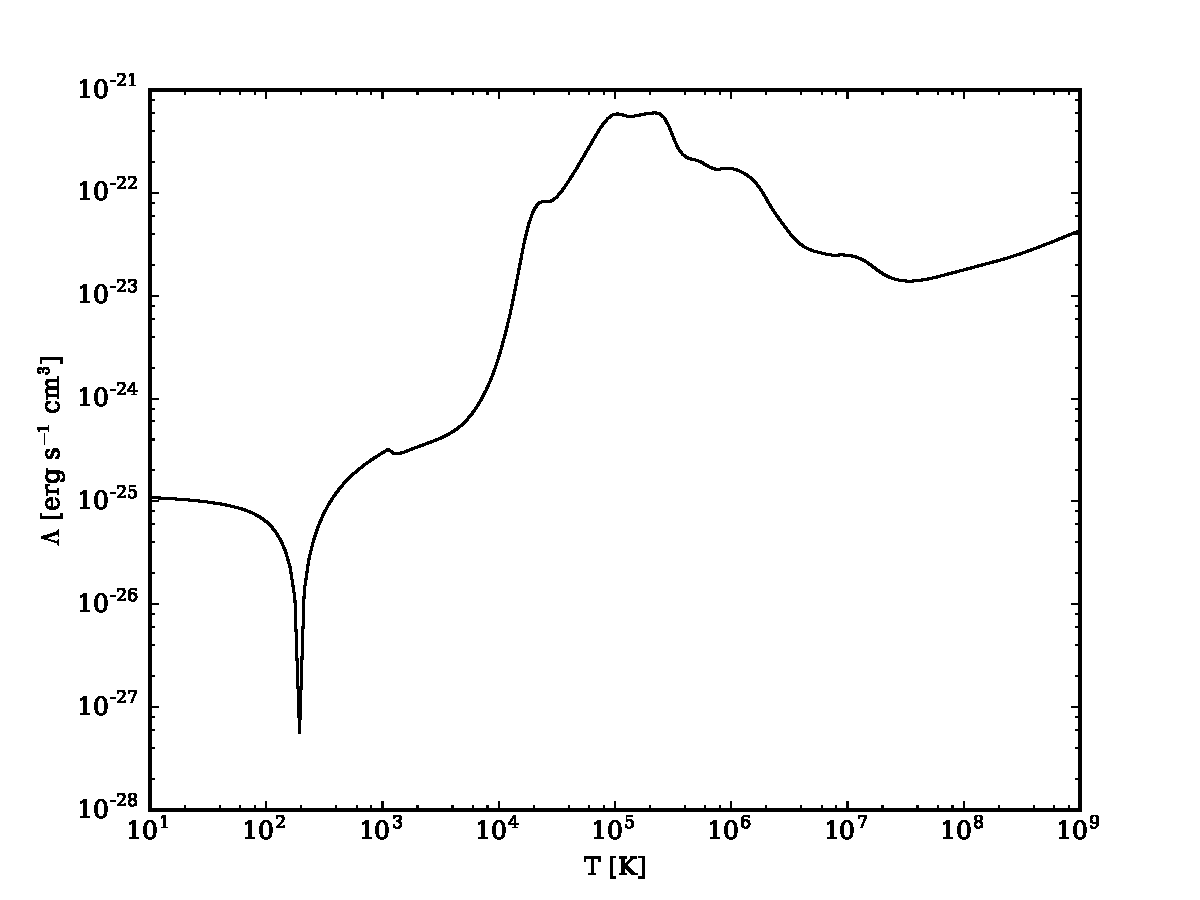
\includegraphics[width=0.45\textwidth]{cooling_rate.pdf}
  \caption{
    Figure output by the default configuration of the cooling rate
    answer test, described in Section \ref{sec:cooling-rate-test},
    showing the equilibrium cooling rate as a function of temperature
    for a solar metallicity gas at a density of 1 amu/cm$^{3}$ with an
    incident radiation field described by the
    \citet{2012ApJ...746..125H} model at z = 0.
  } \label{fig:cooling-rate-test}
\end{figure}

\subsubsection{Answer test: constant density cooling test}
\label{sec:uniform-cooling-test}

The uniform cooling answer test simulates the thermal evolution of a
parcel of gas cooling at constant density.  This test ensures that the
solver properly evolves the internal energy over a period of time.
The test initializes a single-cell fluid container with a density of
0.1 amu/cm$^{3}$ and a temperature of 10$^{6}$ K.  The cell is evolved
for 100 Myr using the \texttt{evolve\_constant\_density} convenience
function with timesteps of 1\% of the cooling time time.  The
resulting evolution is shown in Figure
\ref{fig:uniform-cooling-test}.

\begin{figure}
  \centering
  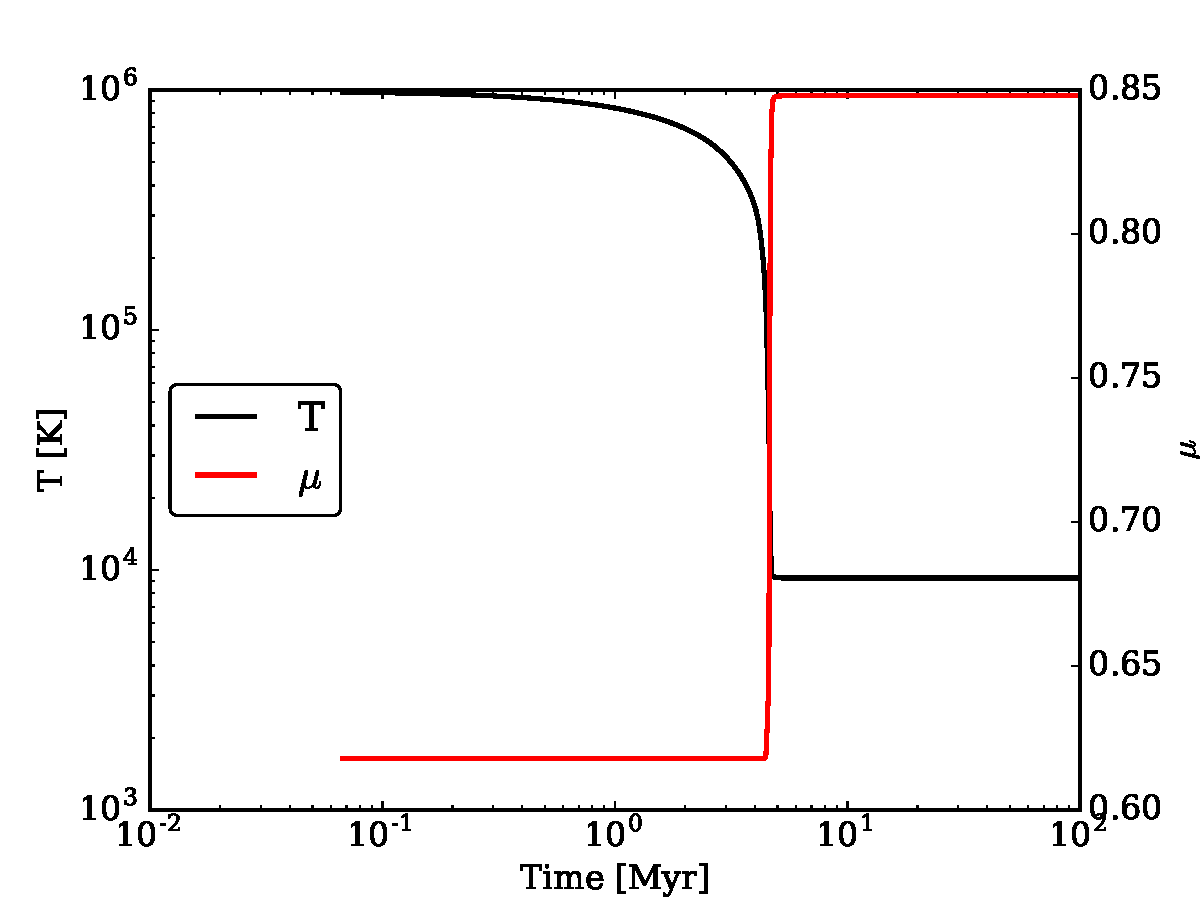
\includegraphics[width=0.45\textwidth]{cooling_cell.pdf}
  \caption{
    Figure output by the uniform cooling answer test, described in
    Section \ref{sec:uniform-cooling-test}, showing the temperature
    (black) and mean molecular weight (red) as a function of time for
    a parcel of gas cooling at constant density.
  } \label{fig:uniform-cooling-test}
\end{figure}

\subsubsection{Answer test: free-fall collapse test}
\label{sec:free-fall-test}

The free-fall collapse answer test simulates the thermal evolution of
a cloud of gas collapsing due to self-gravity.  This test is useful
for ensuring that the non-equilibrium chemistry solver is functioning
properly over a large range in density.  The test creates a
single-cell fluid container with an initial density of 0.1
amu/cm$^{3}$ and an initial temperature of
50,000 K.  Before beginning the free-fall collapse phase, the cloud is
allowed to cool at a constant density to a temperature of 100 K using
the \texttt{evolve\_constant\_density} function described in Section
\ref{sec:pyevolve}.  This allows the gas to settle into an ionization
state that is roughly appropriate for the temperature.  From there, we
evolve the density of the cloud using the \texttt{evolve\_freefall}
function, also discussed in Section \ref{sec:pyevolve}.  This test is
performed using the full non-equilibrium chemistry solver, once at
zero metallicity (Figure \ref{fig:free-fall-test}) and once with a
metallicity of 10$^{-3}$ Z$_{\odot}$.

\begin{figure}
  \centering
  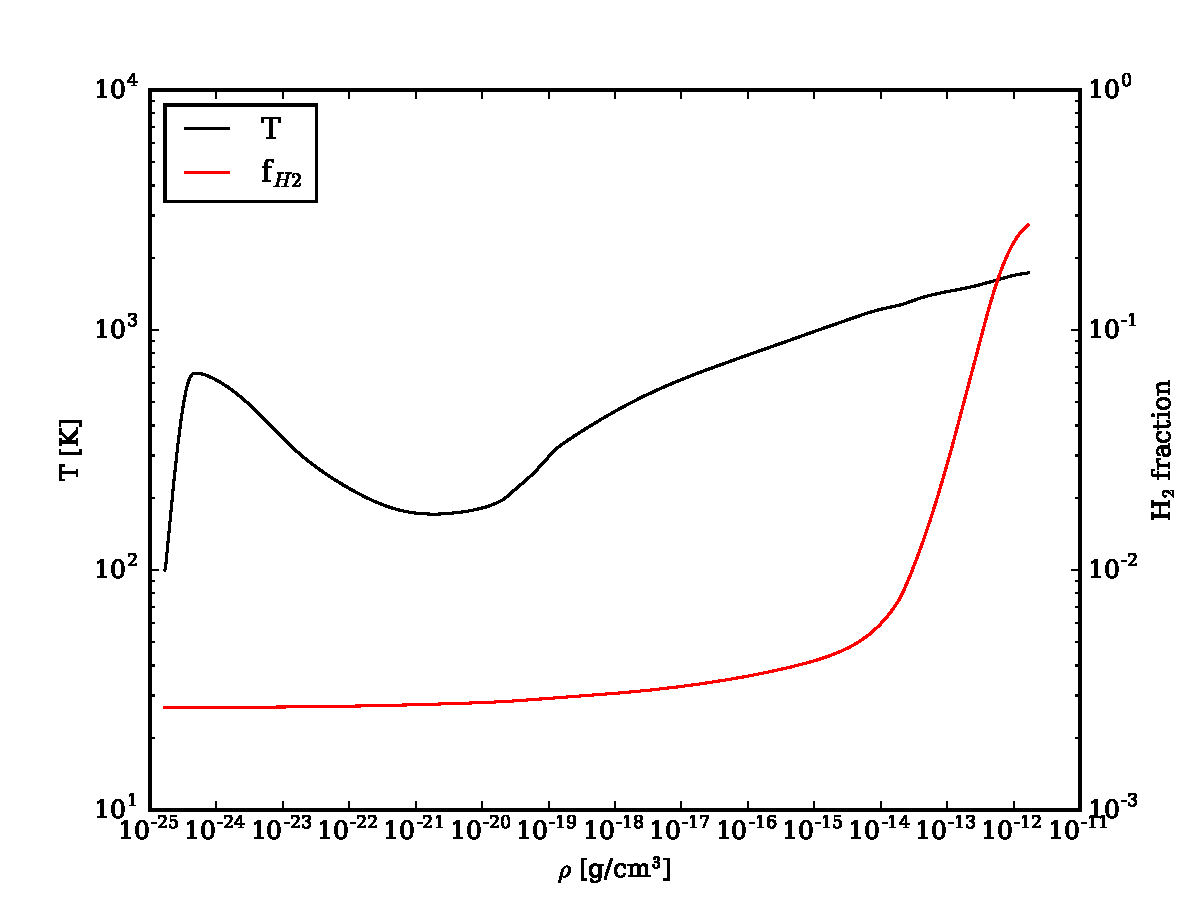
\includegraphics[width=0.45\textwidth]{freefall.pdf}
  \caption{
    Figure output by the default configuration of the free-fall answer
    test, described in Section \ref{sec:free-fall-test}, showing the
    temperature (black) and H$_{2}$ fraction (red) as a function of
    density for a free-fall collapse model of a metal-free gas.
  } \label{fig:free-fall-test}
\end{figure}

\subsection{Performance}


\subsubsection{Optimization Strategy}

Our optimization strategy in the \texttt{Grackle} has two components related to serial and parallel execution.  We begin with single processor optimization.  

The ordinary differential equations that describe chemical and thermal evolution do not use spatial information and so each discretization point (particle or cell) can be evolved independently of the others.  Because of this, the \texttt{Grackle} can be used with a wide variety of codes and applications, and optimization is relatively straightforward.  Our primary technique for single processor optimization is to make good use of cache and (single processor) vectorization.  The API is built around the idea of ``fields" of points (fluid containers) rather than a single point for this reason.  The field can be a single-dimensional contiguous list as might be used for particle-based codes, or a three dimensional grid with inactive ("ghost") points as would be appropriate for grid-based codes.  By taking an entire field, and operating on the field in an order corresponding to the way it is laid out in memory, the code tries to minimize cache misses.  In particular, multi-dimensional arrays are assumed to be fortran-ordered (column-major) and operations are performed in loops over the most rapidly varying index.  Loops are generally also written in a way which facilitates unrolling so that compilers can easily make use of vector operations and prefetching.  Much of the computationally intensive part of the code is written in FORTRAN (in part for historical reasons but in part to take advantage of well-tested FORTRAN compiler loop optimizations).

The second optimization involves taking advantage of parallel computation.  \texttt{Grackle} itself requires no communication and so can easily work as part of a code that uses MPI or some other message passing library to achieve distributed parallelization.  In addition, \texttt{Grackle} supports OpenMP parallelization and thus can easily work with applications adopting a hybrid MPI/OpenMP model.  The OpenMP is implemented by parallelizing over outer j,k loops and giving a thread an i ``slice" to operate on.  This is a natural model for grid-based codes, but some work may be required to get good performance this way with particle based codes (e.g. by artificially splitting a 1D list of particle quantities into a 2D grid).

\subsubsection{Serial Performance}

\begin{figure}
  \centering
  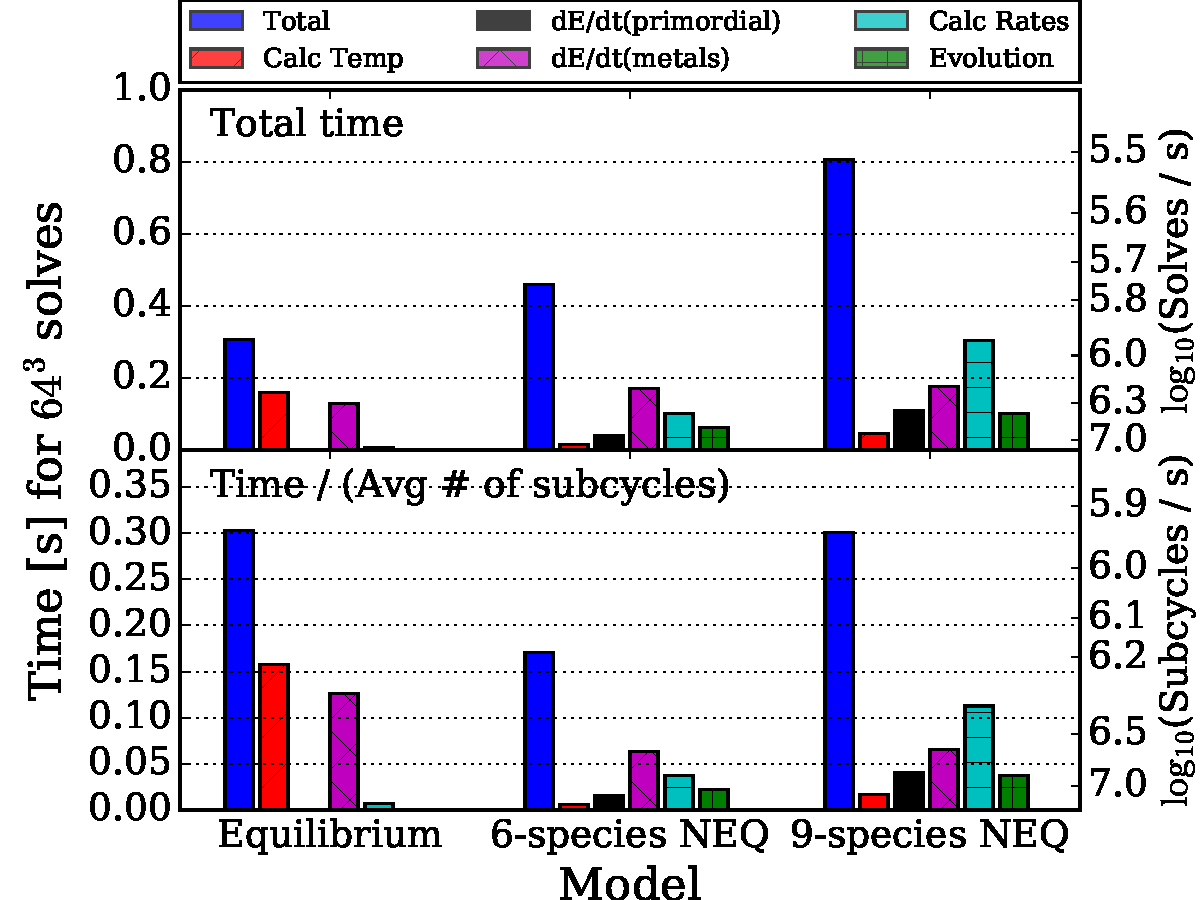
\includegraphics[width=\columnwidth]{performance.pdf}
  \caption{Top panel: Total time to compute the cooling rate test
    (\S\ref{sec:cooling-rate-test}) in $64^3$ fluid containers, using
    the tabulated equilibrium cooling model (left), six species
    non-equilibrium model (middle), and nine species non-equilibrium
    model (right).  The different bars show the time needed for the
    complete solve (blue), the temperature calculation (red), the
    $\dot{e}$ computation due to primordial chemistry (black) and
    metals (magneta), the interpolation of rate coefficients (cyan),
    and the update of the species fractions with backward
    differencing.  Bottom panel: Total time but normalized by the
    average number of subcycles per cell, which demonstrates the
    performance of a single iteration in each solver
    mode.} \label{fig:performance}
\end{figure}

We utilize the cooling rate test (\S\ref{sec:cooling-rate-test}) to
assess the performance of \texttt{Grackle}.  We set up the test with $64^3$
fluid containers with hydrogen number density $n_{\rm H}$, temperature
$T$, and metallicity $Z$ varying in each dimension.  These quantities
are equally log-spaced in the range $\log (n_{\rm H} /
\textrm{cm}^{-3}) = [-1, 3]$, $\log (T/\textrm{K}) = [1, 8]$, and
$\log (Z/Z_\odot) = [-4, 0]$.  All of the fluid containers are
initially neutral.  We run each test with the tabulated solver in
ionization equilibrium and the non-equilibrium solver with the
six species and nine species networks on a single core of a desktop
computer with dual Intel Xeon ``Westmere'' E5645 CPUs at 2.4 GHz, each
of which has six cores.  The tests are evolved for 500 yr, which in
most cases is shorter than the cooling time, however, it provides an
ample test for the performance of \texttt{Grackle}.  Because the fluid
containers are not initialized in ionization equilibrium, the first
timestep in the non-equilibrium solvers requires hundreds of subcycles
for the system to converge.  Due to the fact that the non-equilibrium solver
performance is directly tied to the number of subcycles, we do not
include the first three cycles of the tests (which are not representative of
typical use conditions).

% Something about this is an ideal solve, but performance can diminish
% if more difficult (high densities, shocks, or ionization) conditions
% exist.

The top panel of Figure \ref{fig:performance} shows the total time
(blue bars) required for this $64^3$ performance test in each solver
mode.  This is further divided into the time spent in each major
component of \texttt{Grackle}: the calculation of the temperature (red),
$\dot{e}$ from primordial (black) and metal (magenta) species, rate
coefficient interpolation (cyan), and the update of the species
fractions (green).  From a total performance standpoint, the
non-equilibrium solver in the six species and nine species primordial
models require 50\% and 164\% more time than the equilibrium solver,
respectively.  In this test, \texttt{Grackle} can update $8.6 \times 10^5$,
$5.7 \times 10^5$, and $3.2 \times 10^5$ fluid containers per second
for the equilibrium, six species and nine species solvers, respectively.
The computational expense in the equilibrium solver is almost evenly
split between the equilibrium temperature calculation and metal
cooling rates.  The metal cooling rate and rate coefficient
interpolation consume the most compute cycles in the six species and
nine species solvers, respectively.  The temperature calculation in the
non-equilibrium solver takes relatively little computation because it
is simply calculated from the pressure and total number density with
no iterative processes.

The cooling rate test represents a fluid in many different
chemo-thermal states, which converge to some equilibrium.  However in
production simulations, there are many ``difficult'' situations, such
as high densities, strong shocks, and strong radiation fields, in
which the equations become stiff and require many subcycles to
complete an entire solve.  Therefore to better gauge the performance
of a single iteration, we show the average time elapsed {\it per
  subcycle} for the same test in the bottom panel of Figure
\ref{fig:performance}.  The equilibrium and non-equilibrium solvers
take an average of 1.01 and 2.67 subcycles per solve, respectively.
\texttt{Grackle} can perform $8.7 \times 10^5$, $1.5 \times 10^6$, and $8.7
\times 10^5$ subcycles per second for the equilibrium, six species and
nine species solvers, respectively.  Here we see that the equilibrium
solver actually requires 75\% more time per subcycle as the six species
non-equilibrium solver and is equivalent to the performance (per
subcycle) of the nine species non-equilibrium solver.  In practice, if
any cells require many subcycles to converge to a solution, the call
to \texttt{Grackle} will require additional time per cell than this ideal test,
because the total performance is entirely dependent on the total
number of subcycles performed in one solve, not the number of cells.

\subsubsection{OpenMP Performance}

In addition to the single-processor performance just described, we
characterize the threaded performance of the \texttt{Grackle}.
Figure \ref{fig:omp-perf} shows an OpenMP performance benchmark for both the
non-equilibrium and tabulated functionality, where parallel efficiency is
defined as the ratio of multi-thread to single-thread performance. We
conduct this benchmark on the Campus Cluster of the University of Illinois
at Urbana-Champaign using 20 threads on two Intel Xeon E5-2670 v2 CPUs
at 2.50 GHz, each of which has ten cores. For all time-consuming routines
(i.e., calculating cooling, cooling time, and temperature with the tabulated
solver, and calculating chemistry, cooling, and cooling time with the
non-equilibrium chemistry solver), the parallel efficiency reaches
$\sim 60\%\,\text{--}\,90\%$ for $16^3$ cells and
$\sim 80\%\,\text{--}\,90\%$ for $64^3$ cells. For other computationally cheap
routines, such as calculating pressure, the parallel efficiency is relatively
low. This is not an issue since they take negligible time compared to other
computationally expensive routines.

\begin{figure}
  \centering
  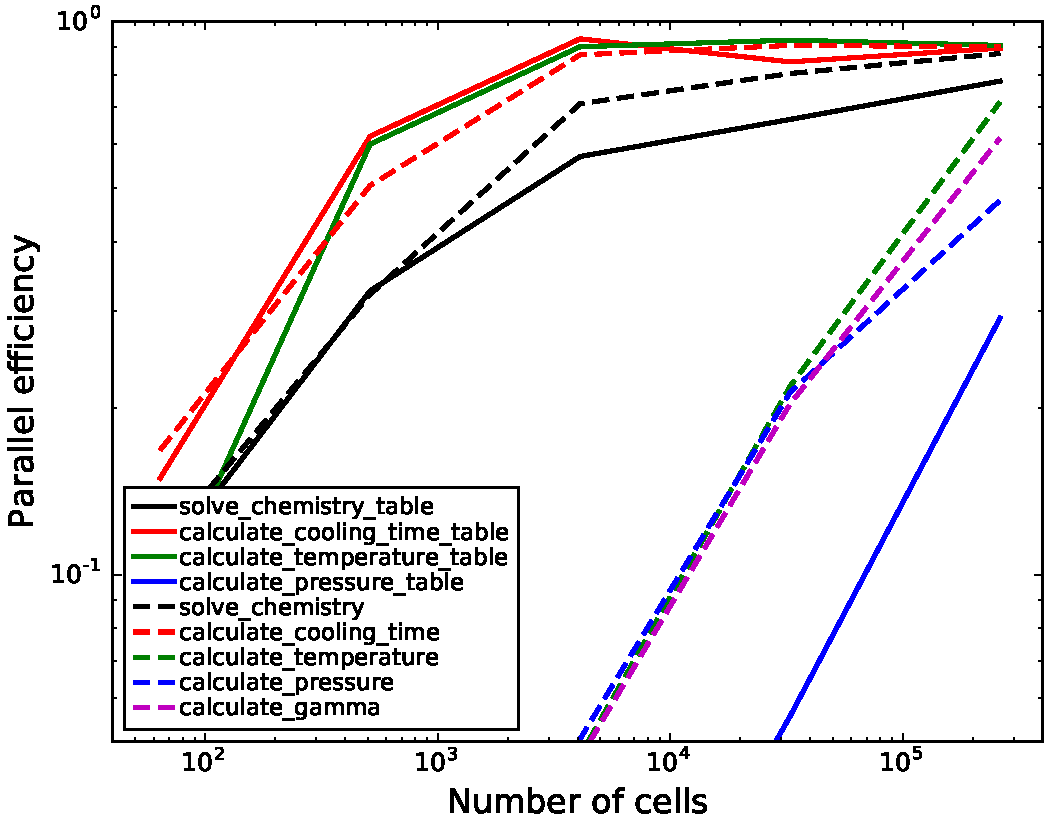
\includegraphics[width=0.45\textwidth]{fig__openmp_performance.pdf}
  \caption{
    OpenMP parallel efficiency using 20 threads as a function of the size of
    the input array. The solid lines show the use of the
    non-equilibrium solver with \texttt{primordial\_chemistry} = 3 and
    the dashed lines show the analogous functions using the tabulated
    solver.  For all time-consuming
    routines, the parallel efficiency reaches $\sim$60\% to 90\% for
    $16^3$ cells and $\sim$80\% to 90\% for $64^3$ cells.
  } \label{fig:omp-perf}
\end{figure}

%%% Local Variables:
%%% mode: latex
%%% TeX-master: "ms"
%%% End:


\section{Summary} \label{sec:summary}

\subsection{Applicability and Limitations}

It is important to remember that the range of physical conditions in
which Grackle can be considered valid is not unlimited.  In Figure
\ref{fig:valid-range}, we show the rough density range over which
different components of the solver is valid.  The high density limit
of the non-equilibrium solver is set roughly by the reactions present
in the network and the range over which their rate coefficients are
trusted.  The limits on the cooling tables correspond to the density
range over which they were calculated.  Users are especially
cautioned against exceeding the upper density limit of the tabulated
cooling solver.  The critical density above which energy levels are
populated according to LTE exceeds the upper limit of the tables for
many metal coolants \citep{2008MNRAS.385.1443S}.  Thus, these tables
do not capture the NLTE to LTE transition where the cooling rates
change from scaling as $\rho^{2}$ to $\rho$.  Hence, extrapolation
beyond the upper limit may result in vast over-prediction of the
cooling rate.  If the use-case requires exceeding this limit, then the
high density metal table should be used in conjunction with the
non-equilibrium solver.  It is also extremely important to remember
that all Grackle calculations are based on the assumption that the
medium is optically thin.  In practice, the length scale of optical
thickness will become very short as density increases.

\begin{figure}
  \centering
  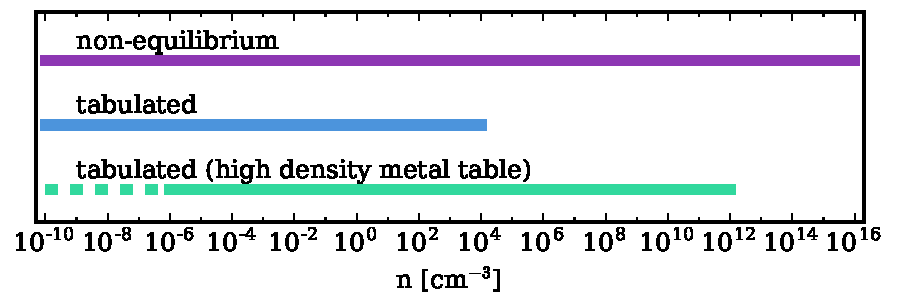
\includegraphics[width=0.48\textwidth]{valid_range.pdf}
  \caption{
    The appropriate density range for different versions of the
    Grackle solver.  The high density metal cooling table (bottom)
    explicitly spans the density range, 10$^{-6}$ cm $^{-3}$ $< n <$
    10$^{12}$ cm $^{-3}$, but extrapolation down to $n = 10^{-10}$ cm
    $^{-3}$ is still valid, as indicated by the dashed line.  For each
    of these, the valid temperature range is roughly 1 K to 10$^{9}$
    K.
  } \label{fig:valid-range}
\end{figure}

The addition of radiative cooling to a simulation creates another
relevant length scale which must be kept in mind.  The cooling length,
defined as the product of the local sound speed and the cooling time,
sets the approximate size of objects as they cool and condense
\citep{2009A&A...508..725I}.  The cooling length is inversely
proportional to density, effectively setting a density limit for
any given spatial resolution.  When this scale becomes unresolved,
radiative losses will be overpredicted, leading to unphysically high
densities and further exacerbating the resolution problem in a runaway
cycle.  This effect is likely related to the over-cooling problem that
has classically plagued cosmological simulations
\citep[e.g.][]{1996ApJS..105...19K, 2001MNRAS.326.1228B}.
In Figure \ref{fig:cooling-length}, we show an estimate of the
cooling length for the scenario of a gas at solar metallicity in a
\citet{2012ApJ...746..125H} radiation background at z = 0, noting how
quickly the cooling length drops below 1 kpc, and even 1 pc, for
densities relevant to galaxy formation simulations.  This
length scale should be taken into consideration when choosing the
density threshold above which sub-grid models are applied.

\begin{figure*}
  \centering
  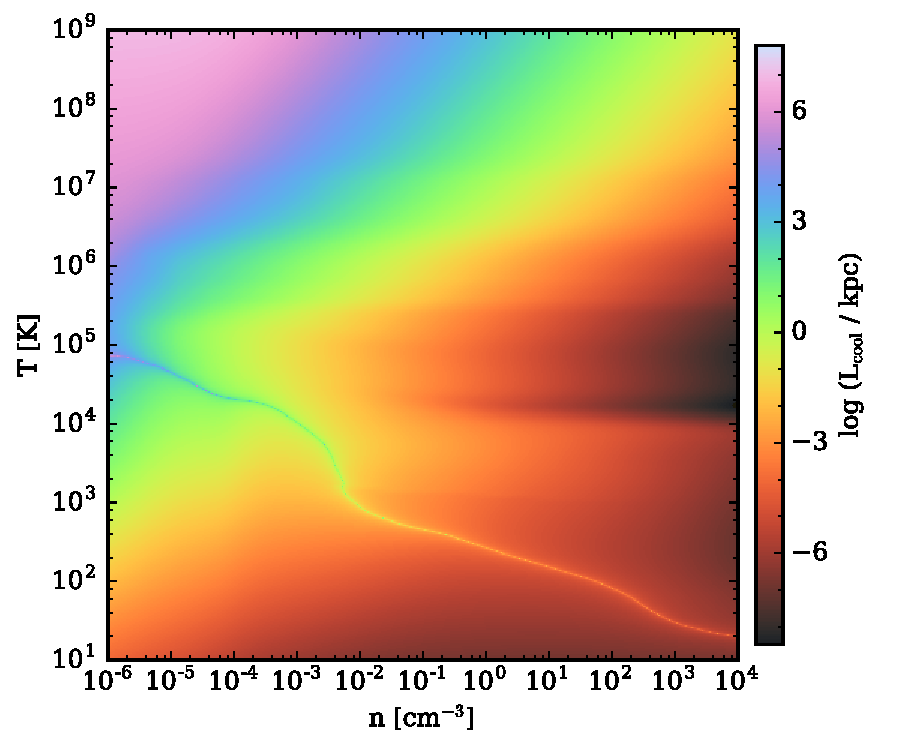
\includegraphics[width=0.84\textwidth]{cooling_length.pdf}
  \caption{
    The cooling length, defined as the product of the Jeans length and
    the cooling time, as a function of number density and temperature
    for a gas with solar metallicity exposed to a radiation field
    defined by the model of \citet{2012ApJ...746..125H} at z = 0.  The
    narrow line extending from the middle, left to the bottom, right
    represents the temperature where heating and cooling are
    balanced.  Above this line, the gas is being cooled while below
    the line it is being heated.
  } \label{fig:cooling-length}
\end{figure*}

\subsection{Simulation codes with Grackle}
To date, the following codes are known to have \texttt{Grackle}
implemented:
\begin{itemize}

\item AREPO \citep{2010MNRAS.401..791S}

\item ART-I \citep{1999PhDT........25K, 2002ApJ...571..563K}

\item ART-II \citep{2008ApJ...672...19R}

\item CHANGA \citep{2004NewA....9..137W, 2006MNRAS.373.1074S}

\item Enzo \citep{2014ApJS..211...19B}

\item Gadget-3 \citep{2005MNRAS.364.1105S}

\item GAMER \citep{2010ApJS..186..457S}

\item GASOLINE \citep{2004NewA....9..137W}

\item Gear \citep{2012A&A...538A..82R, 2012ASPC..453..141R}

\item Gizmo \citep{2015MNRAS.450...53H}

\item RAMSES \citep{2002A&A...385..337T}

\end{itemize}

\subsection{Future Directions} \label{Future_Directions}

\subsubsection{Including new rates and models in Grackle}
The current code structure is highly integrated. This makes introducing new rates for the 
chemical network or cooling network a rather intricate task requiring multiple changes throughout the code. 
Apart from the fact that this is more time consuming it is also much more error prone. In a future release of the 
code the modularity of the code will be increased greatly. There will be a function to populate the species 
rate coefficients and a function to populate the cooling coefficients. Separate template files can then be 
updated by a developer wishing to use their own rates. This file can then be included in the build and a flag
set to indicate the new rates be used in place of the old rates. Furthermore, a similar method will be 
implemented for solving the network. A template network solver will be available which the developer can use to 
implement a new network with a developer determined number of species. The developer will be responsible for
updating only three files to achieve a solution to their own chemical network. 

\subsubsection{Connection to Radiative Transfer}

As discussed in \S\ref{section:radback}, Grackle includes the effects
of a radiation background that can ionize, heat, and dissociate atoms
and molecules through the radiative reaction and destruction rates in
Equations (\ref{eq:rate_general}) and (\ref{eq:rateCD}), respectively.
Because photo-effects are already implemented into the network, it will
be relatively trivial to couple Grackle with a radiation transport
solver.  Here, Grackle would accept additional spatially-varying
fields of photoionization rates, photoheating rates, and
photodissociation rates to add to or replace the background radiation
values.  All of the heavy computation calculating these radiation
fields is accomplished by the transport solver, whether it be through
a Monte Carlo or moment method.  Grackle can be called in radiative
transfer codes that are either called in post-processing, usually for
cosmic reionization calculations \citep[e.g.][]{2014MNRAS.439..725I,
  2016MNRAS.459.2342M}, or coupled with the hydrodynamics, which is
becoming more commonplace in galaxy and star formation simulations
\citep[e.g.][]{2014MNRAS.442.2560W, 2015MNRAS.451...34R,
  2015arXiv151100011O, 2015MNRAS.454..380B, 2016arXiv160300034P, 2016arXiv160703117R}.
Additional connections to radiative transfer models could use the
local radiation intensity instead of spatially invariant values.  Some
examples include a more accurate computation of (i) the photoelectric
effect, (ii) the heating and cooling rates from metals, where the
local UV/X-ray flux would be an additional interpolation variable in
the lookup table, and (iii) the self-shielding of a UV background.

\subsubsection{Multiple element cooling}

Currently, \texttt{Grackle} only considers a single metallicity field
for the calculation of the cooling due to heavy elements.  However,
more sophisticated feedback models now consider feedback from multiple
sources, like type Ia and type II supernova and winds from AGB stars,
each of this producing distinct abundance patterns.  In the future, we
will look to create additional cooling tables that consider varying
abundance patterns.  As an intermediate step before creating cooling
tables for every metal species, as in \citet{2009MNRAS.393...99W}, we
will likely begin with a two-element model distinguishing between type
Ia and II supernovae, such as that of \citet{2013MNRAS.433.3005D}.



%%% Local Variables:
%%% mode: latex
%%% TeX-master: "ms"
%%% End:


\section*{Acknowledgements}

BDS would like to thank the organizers of the AGORA project, Ji-hoon
Kim, Joel Primack, and Piero Madau for the original motivation for the
\texttt{Grackle} project as well as Nick Gnedin, James Wadsley, and
Romeel Dav$\acute{\rm e}$ for providing useful suggestions for
additional functionality.  GLB acknowledges support from
NASA grant NNX15AB20G and NSF grant 1312888.  We also thank the NSF
for computational resources provided through the XSEDE program.


%%%%%%%%%%%%%%%%%%%%%%%%%%%%%%%%%%%%%%%%%%%%%%%%%%

%%%%%%%%%%%%%%%%%%%% REFERENCES %%%%%%%%%%%%%%%%%%

\footnotesize{
  \bibliographystyle{mnras}
  \citestyle{mnras}
  \bibliography{ms}
}

\bsp
\label{lastpage}
\end{document}
